\chapter{Implementace}
\label{implementation}
\emph{Implementační} část práce se skládala z několika součástí. Za nejvýzamnější součást lze považovat formální specifikaci pravidla \emph{Law of Demeter}, která je uváděna jako první v rámci této sekce. V dalších částech kapitoly se potom zabýváme vybranými poznámkami z implementace jádra systému ArchVal, který má sloužit jako platforma pro provádění matematických formulací návrhových pravidel a implementací rozšíření tohoto systému. V poslední části je rozebírán způsob integrace systému do platformy NetBeans.

\section{Specifikace pravidel požadovaných zadáním práce}
Nejprve definujeme vhodné operátory, které nám umožní vybrat množiny vrcholů tak, abychom mohli specifikova LoD. Vybrané množiny potom ověříme pomocí predikátu, který určí, zda jsou tyto množiny v~pořádku, či zda porušují \emph{LoD} princip.

\begin{definition}
Mějme grafový model projektu $G = \langle V, E, \rho, K, C, N, \mathit{Kind}, \mathit{Classifier}, \mathit{Name}\rangle$. Definujme selektor vrcholů $L_0(G, v', c')$, $v' \in V$, $c' \in C$ jako množinu vrcholů $v \in V$, které jsou přímými následníky vrcholu $v'$, do kterých se dostaneme po hraně $e \in E$, pro kterou platí $Classifier(e) = c' $.
\end{definition}

\begin{definition}
Mějme grafový model projektu $G = \langle V, E, \rho, K, C, N, \mathit{Kind}, \mathit{Classifier}, \mathit{Name}\rangle$. Definujme selektor vrcholů $L_1(G, v', c_1, c_2)$, $v' \in V$, $c_1 \in C$, $c_2 \in C$ jako množinu vrcholů $v \in V$, do nichž se dostaneme z vrcholu $v'$ po orientované cestě délky 2, pro jejíž první hranu $e_1$ platí $Classifier(e_1) = c_1$ a pro druhou hranu $e_2$ platí $Classifier(e_2) = c_2$.
\end{definition}

\subsection{Law of Demeter}
\label{implementation-lod_specification}
Pro definici princip LoD si zavedeme speciální typ grafového modelu. Ačkoliv jsme pojem \emph{typ grafového modelu}  přesně nedefinovali a zavedli jej pouze intuitivně, pokusíme se nyní vymezit pojem \emph{demeter graph model}, který zde budeme dále používat, přesněji.

U grafového modelu typu \emph{Demeter graph type} povolíme libovolná označení vrcholů (konkrétně pro potřeby LoD se bude jednat o plně kvalifikované názvy tříd a metod). Množinu typů vrcholů omezíme na následující množinu:
\begin{align*}
K = \{ ``class", ``method" \}
\end{align*}
Význam těchto typů je zřejmý. Typ \emph{class} použijeme pro vrcholy, které budou odpovídat deklarovaným třídám v existujícím projektu a typ \emph{method} bude označovat jejich metody.

Taktéž množina klasifikátorů hran nebude libovolná, ale bude přesně daná:
\begin{align*}
C = \{ ``field", ``self", ``arg", ``constr", ``use" \}
\end{align*}
Podívejme se na význam těchto označení:
\begin{itemize}
\item $``field"$ -- hrana vede do třídy, které reprezentuje třídní promenou nebo do její nadtřídy
\item $``self"$ -- hrana vede do třídy, která je vlastníkem této metody nebo do její nadtřídy
\item $``arg"$ -- hrana vede do třídy argumentu metody nebo do její nadtřídy
\item $``constr"$ -- hrana vede do třídy použité pro konstrukci nového objektu v těle metody nebo do její nadtřídy
\item $``use"$ -- hrana vede do třídy, jejíž použití (vyvolání metody nebo přístup k poli) se vyskytuje v těle metody
\end{itemize}
Je patrné, že tyto hrany zčásti odpovídají požadavkům LoD. Prozatím jsme uvedli množiny klasifikátorů bez vymezení, kde lze přesně tyto klasifikátory použít. Uvažujme následující množinu, která reprezentuje zobrazení množiny klasifiktároů do množiny dvojic typů vrcholů:
\begin{align*}
GT = &\{ \\
&(``field" (``class", ``class")), \\
&(``self" (``method", ``class")), \\
&(``arg" (``method", ``class")), \\
&(``constr" (``method", ``class")), \\
&(``use" (``method", ``class")) \\
&\}
\end{align*}
Pokud budeme uvažovat koncové vrcholy jednotlivých hran a jejich zobrazení do množiny typů, potom musí platit, že obraz jednotlivých komponent hrany (vrcholů) bude shodný s~obrazem hrany provedeného pomocí zobrazení GT.

Pokud \emph{grafový model projektu} splní všechny tyto podmínky, řekneme o něm, že je typu \emph{demeter}.

Příklad takového grafu je na obrázku \ref{implementation-lod_graph}. V~uvedeném obrázku princip LoD porušuje metoda \verb-method1_2-, která používá třídu \verb-Class2-, ačkoliv není ani jednou z dovolených tříd principu LoD (třída pole vlastnické třídy metody, argument metody, atd.).

\begin{figure}[h!]
  \centering
  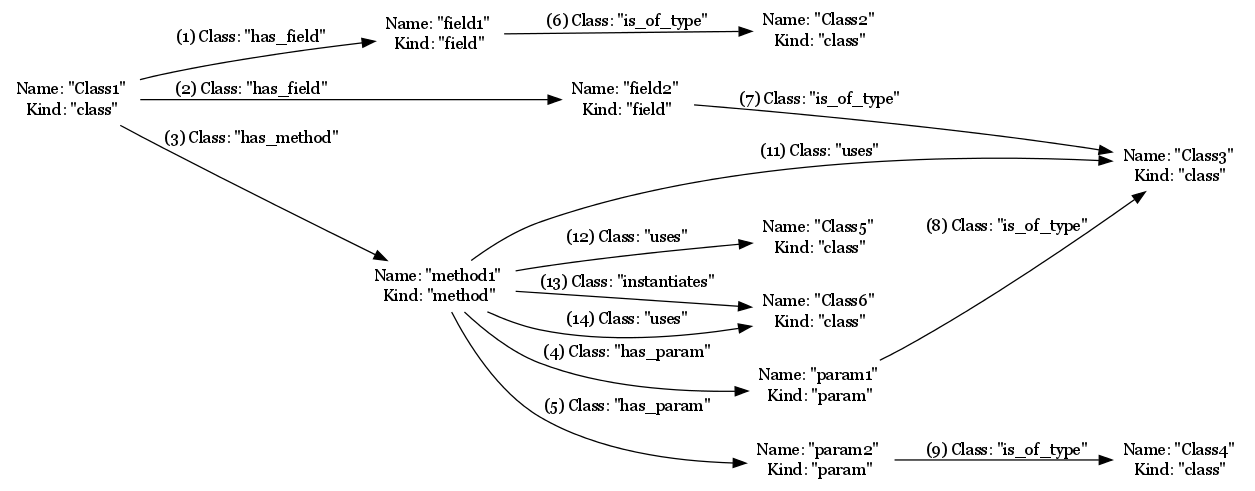
\includegraphics[width=1.0\textwidth]{./graphs/demeter_graph.png}
  \caption{Graf \uv{typu demeter} použitý pro validaci principu LoD.\label{implementation-lod_graph}}
\end{figure}

\begin{designprinciple}
Mějme grafový model projektu $G = \langle V, E, \rho, K, C, \mathit{Kind}, \mathit{Classifier}\rangle$ typu demeter. Model $G$ splňuje návrhový princip LoD, pokud pro něj platí:

\begin{align*}
\forall v \in V: Kind(v) = ``method"\\
\end{align*}
\begin{align*}
&L_0(G, v, ``use") \setminus (G, L_0(v, ``self") \cup L_1(G, v, ``self", ``field") \cup \\
&L_0(G, v, ``arg") \cup L_0(G, v, ``constr")) = \emptyset
\end{align*}

\end{designprinciple}

Specifikované pravidlo vyjadřuje požadavek, aby množina vrcholů (představujících třídy) do níž se dostaneme pomocí hran s klasifikátorem $``use"$ (všechna použití tříd uvnitř metody) byla podmnožinou sjednocení vrcholů, které pro danou metodu představují povolená použití tříd (vlastní třída metody, třída třídní proměnné, argument metody nebo konstruovaná třída). Je-li totiž množina ``use" vrcholů podmnožinou sjednocení ostatních množin, množinový rozdíl bude roven prázdné množině. V opačném případě bude množinový rozdíl nenulový, což bude znamenat porušení principu LoD.

\subsection{Low coupling, high cohesion}
Zatímco princip LoD se nám podařilo přesně specifikovat pomocí množin. U principů \emph{low coupling} a \emph{high cohesion} bychom spíše uvažovali o realizaci vhodné analýzy. Tyto analýzy však nebyly cílem této práce.

Přesto byla realizována programová podpora, která umožní snadné přidání modulu, který může pracovat nad libovolným grafem poskytovaným některým z existujících poskytovatelů generátorů grafů a tyto nebo jiné podobné vlastnosti analyzovat.

Konkrétní informace a rešeše týkající se těchto principů byly rozebrány v kapitole \ref{analysis}.

\section{Implementace jádra systému}
Jádro systému bylo implementováno v rámci samostatného modulu platformy NetBeans. Ačkoliv je takto svázáno s konkrétní platformou, zdrojové kódy neobsahují žádné závislosti na prvky této platformy a je tedy možné je znovupoužít v jiných projektech.

V této sekci nebudeme procházet úplně všechny implementované komponenty systému. Jednak byly popsány již v části návrhu a kromě toho jsou jejich implementace k dispozici v rámci zdrojových kódů. Při implementaci byla snaha o maximální zdokumentovanost -- většina klíčových tříd je řádně opatřena dokumentací \verb-Javadoc-.

Zde se podíváme na implementaci formátu pro zadávání pravidel (AVD specifikace). Dále na způsob sestavování vyhodnocovacího stromu a nakonec ukážeme implementaci zajímavých operátorů, které jsou základem systému pro vyhodnocování pravidel.

\subsection{Implementace formátu AVD}
Formát AVD byl vytvořen snahou o namapování dříve definovaných matematických výrazů do vhodné serializace. Pro zpracování existujícího souboru byl použit lexikální a syntaktický analyzátor vygenerovaný pomocí nástroje ANTLR. Tento nástroj umí kromě vytvoření čistého \emph{parse tree} vytvořit i vhodný AST pomocí jednoduchých přepisovacích pravidel (konkrétní příklady pravidel si můžete prohlédnout v příloze \ref{avd_grammar}, kde je pro refrenci uvedna celá vstupní gramatika pro nástroj ANTLR).

V rámci AVD specifikace bylo nutné definovat několik nezávislých jmenných prostorů:

\begin{itemize}
\item názvy analýz
\item jména typů grafů
\item jména atomických a složených pravidel (jmenný prostor pro atomická i složená pravidla je sdílený)
\item jména operátorů
\end{itemize}

Proto je například možné použít stejný název pro typ grafu a pro atomické pravidlo, ale není možné použít shodný název pro dvě pravidla (ať už atomická nebo složená).

\subsection{Implementace sestavování validačního modelu}
Na základě AST, který byl získán pomocí syntaktického parseru vygenerovaného pomocí nástroje ANTLR byl postupně budován vyhodnocovací strom odpovídající zpracovávanému AVD souboru.

Zpracování AST probíhá tím způsobem, že je nejprve zkontrolována bezkoliznost použitých jmen (viz výše zmíněné jmenné prostory). Následně jsou procházeny jednotlivé listy představující pravidla a jsou postupně doplňovány názvy nalezených pravidel do tabulky symbolů. Pro každé pravidlo je nutné sestoupit do syntaktických stromů představujících např. logické výrazy a pro každý takto nalezených vrchol (např. operátor OR) je nutné vytvořit nový vrchol vyhodnocovacího stromu.

Tyto nově vytvářené vrcholy jsou realizované pro základní operátory jako samostatné třídy. Pro uživatelské operátory potom existují vrcholy, kterým je při konstrukci možné nastavit operátor, který mají provádět. Předtím, než jsou ale tyto vrcholy vytvořeny, je provedena kontrola, zda počty argumentů a návratová hodnota odpovídá očekávaným hodnotám (např. při zpracování predikátu kontrolujeme, zda množina operandů odpovídá množině deklarované operátorem nalezeným v registru operátorů.).

Při budování stromu je současně budována infrastruktura pro generování stromu výsledků. V každém pridáváném vrcholu (představován třídou) je tedy již přítomen kód, který při vyhodnocení uzlu (metoda \verb-evaluate()-) naplní datovou strukturu předanou jako parametr.

\subsection{Implementace základních operátorů}
V této podsekci se podíváme na některé zajímavé operátory a jejich implementaci. Konkrétně na existenční $\exists$ a univerzální $\forall$ kvantifikátor.

Vyhodnocení univerzálního kvantifikátoru $\forall v \in V$ lze přepsat jako jednoduchý cyklus přes vrcholy vrácené zpřesňující operátorem, která vybírá nějakou podmnožinu z~množiny vrcholů analyzovaného grafu. Získáme tak kód podobný listingu \ref{listing-forall}. V~tomto kódu, který je fragmentem metody, používáme symoblický název \verb+condition+ pro podmínku, kterou musí splňovat každý prvek \emph{v} iterované kolekce vrcholů \emph{vertices}.

\begin{lstlisting}[
    language=java,
    caption={Implementace univerzálního kvantifikátoru $\forall$.},
    label=listing-forall
  ]
for (Vertex v : vertices) {
    if (!condition(v, ...)) {
        return false;
    }
}
return true;
\end{lstlisting}

Analogicky budeme postupovat u~existenčního kvantifikátoru $\exists$. Zde nám stačí nalézt alespoň jeden element, pro který vyhodnocovaná vlastnost platí. Listing \ref{listing-exists} představuje fragment metody. Pokud se podaří nalézt alespoň jeden prvek, který splňuje požadovanou podmínku, metoda vrátí hodnotu \emph{true}. Vzhledem k~použití příkazu \emph{return} je zřejmé, že dochází k~\uv{línemu} vyhodnocování -- vyhodnocení je ukončeno nalezením prvního vyhovujícího elementu (další se neprohledávají). Stejně jako u~operátoru $\forall$ i zde název \verb+condition+ symbolizuje konkrétní podmínku, která má platit nad alespoň jedním prvkem množiny uzlů.

\begin{lstlisting}[
    language=java,
    caption={Implementace existenčního kvantifikátoru $\exists$.},
    label=listing-exists
  ]
for (Vertex v : vertices) {
    if (condition(v, ...)) {
        return true;
    }
}
return false;
\end{lstlisting}

Můžeme si všimnout, že se obě implementace liší pouze přehozením podmínek -- zatímco v~prvním případě ($\forall$) musíme projít všechny prvky, abychom zjistili, zda všechny prvky splňují požadovanou vlastnost, ve druhém případě ($\exists$) budeme všechny prvky procházet pouze v~krajním případě, kdy vlastnost neplatí pro žádný z~prvků.

Podobným způsobem jsou realizovány i další operátory. Například sjednocení množin využívá operací poskytovaných třídou \verb-HashSet- programovacího jazyka Java.

\section{Implementace modulů rozšíření}
V rámci této práce byly realizovány celkem dva netbeans moduly realizující rozšíření. Tyto moduly mohou současně sloužit jako návod k implementaci dalších rozšíření. Jedná se o poskytovatele generátoru grafu typu \emph{demeter} a balíček operátorů, které jsou nezbytné k provedení pravidla \emph{LoD}. Tyto operátory nicméně nejsou vázány pouze na princip \emph{Law of Demeter}. Například operátor, který testuje, zda je množina vrcholů prázná má zcela jistě obecné použití.

\subsection{Modul av-graphgen-demeter (generátor grafu)}
Modul pro generování grafu nad nímž je možné provést kontrolu principu LoD, je realizován díky možnosti využít existující infrastrukturu platformy NetBeans pro práci se zdrojovými kódy v jazyce Java a jejich syntaktickými stromy. Jak již bylo zmíněno dříve v rámci analýzy, platforma NetBeans poskytuje AST stromy, které mají již rozlišené symboly. Díky tomu můžeme stromy postupně procházet a dotazovat se na plně kvalifikovaná jména elementů představujících třídy, rozhraní atd.

Generátor grafu je realizován v rámci třídy \emph{DemeterGraphGenerator} (implementuje rozhraní \emph{GraphGeneratorIface}). Protože vstupním parametrem pro generátor grafu je \uv{pouze} adresář projektu. Je nutné vylistovat všechny soubory, které mohou obsahovat zdrojový kód v jazyce Java (\verb+*.java+ soubory). Následně je pro každý takový soubor získána instance třídy \emph{JavaSource} poskytované platformou NetBeans. Tato třída je vstupním bodem k funkcionalitám poskytovaným kompilátorem jazyka Java (třída JavaSource tato rozhraní zabaluje). Díky tomu je možné využít \emph{Java Tree API} pro iteraci všech syntaktických elementů v rámci kompilační jednotky.

To je provedeno formou návrhového vzoru \emph{Visitor}. Při generování demeter grafu nemusíme naštěstí přepisovat všechny metody třídy \emph{TreePathVisitor}, ale zaměřujeme se pouze na elementy, které potřebujeme pro vygenerování grafu. Pro vygenerování potřebného grafu nám stačí získat následující informace: které třídy je metoda členem, zjištění všech nadtříd třídy, konstrukce nové proměnné (nebo pole proměnných), deklarace polí třídy, vyvolání metody a přístup k poli třídy. Ostatní syntaktické konstrukce nejsou pro tento druh generování grafu podstatné.

\subsection{Modul av-operators-demeter (operátory pro LoD)}
Balík operátorů poskytovaný modulem \verb+av-operators-demeter+ obsahuje následující operátory:

\begin{itemize}
\item \verb+vertex_set_is_empty+ -- třída \emph{EmptyVertexSetPredicate} -- operátor, který vrátí \verb+true+ v případě, že je množina vrcholů předaná jako parametr prázdná
\item \verb+level_zero_vertex_selector+ -- třída \emph{LevelZerorVertexSelector} -- implementace operátoru $L_0$ tak jak byl definován dříve
\item \verb+level_one_vertex_selector+ -- třída \emph{LevelOneVertexSelector} -- implementace operátoru $L_1$ tak jak byl definován dříve
\item \verb+kind+ -- třída \emph{VertexKindPredicate} -- predikát, který vrátí \verb+true+, pokud má vrchol předaný jako první parametr typ shodný s řetězcem předaným jako druhý parametr
\end{itemize}

Implementace oprátorů je poměrně přímočará. Zajímavý je snad jen operátor \emph{F}, který pomocí jednoduché rekurze implementuje modifikované prohledávání do hloubky, aby získal množinu potřebných vrcholů.

\section{Integrace do NetBeans IDE}

Pro demonstraci jádra systému bylo nutné jej zaintegrovat do vhodného běhového prostředí. K tomu dobře posloužila platforma NetBeans. Při implementaci bylo hojně využíváno informací z~\cite{netbeans_platform}. Integrace byla provedena realizací vhodných integračních komponent v rámci modulu \verb+av-platform-integration+. Jejich seznam je k~dispozici v~tabulce \ref{implementation-integration_components}.

\begin{table}
  \caption{Tabulka integračních komponent systému. \label{implementation-integration_components}}
  \begin{center}
    \begin{tabular}{ | l | l | p{8cm} | }
      \hline
      \textbf{Název} & \textbf{Typ} & \textbf{Zodpovědnost} \\
      \hline
      \hline
      ArchvalInstance & class (singleton) & zabaluje jednotnou instanci jádra Archval \\ \hline
      ValidateMainProject & class & integrace s~běhovou platformou, vstupní/aktivační bod \\ \hline
      GraphGeneratorRegister & class & třída poskytující přístup k~informacím o~existujících poskytovatelích generátorů grafu \\ \hline
      OperatorRegister & class & třída poskytující přístup k~informacím o~existujících poskytovatelích operátorů \\ \hline
      AnalysesRegister & class & třída poskytující přístup k~informacím o~existujících poskytovatelích komponent analýzy \\ \hline
    \end{tabular}
  \end{center}
\end{table}

\subsection{Použití jádra systému ArchVal}
Vstupním bodem pro použití rozhraní jádra systému ArchVal v rámci integračního modulu je třída \emph{ArchvalInstance}. Tato třída je implementována jako návrhový vzor \emph{singleton} a poskytuje jedinou instanci třídy \emph{ArchVal} pro celý systém. Díky tomu je možné se dále dostat k důležitým komponentám jako \emph{ValidationModelGenerator}, \emph{GraphModelGenerator} a vygenerovat instanci \emph{ValidationTask}, která umí provést výslednou validaci.

\subsection{Přidání uživatelské akce do nabídky prostředí}
Aby bylo možné vyvolat validaci, bylo nutné provést integraci akce do nabídky Netbeans IDE. Akce představovaná třídou \emph{ValidateMainProject} byla realizována jako podmíněně povolená akce, která je k dispozici pouze pokud je vybrán soubor konkrétního typu. V tomto případě se jedná o soubor typu AVD. Celý případ užití funguje potom tím způsobem, že uživatel klepne pravým tlačítkem na AVD soubor a vybere položku \emph{Validate main project}. Pokud není žádný projekt vybrán jako hlavní, v oznamovací oblasti se pouze objeví upozornění a není provedena žádná akce. V opačném případě máme k dispozici oba vstupy potřebné k provedení validace (pomocí \emph{Project API} získáme informace o hlavním projektu a tedy i vstupním adresáři a cesta k AVD souboru je poskytována v rámci handleru kontextové akce AVD souboru).

\subsection{Výstupní rozhraní}
Pro zobrazení výstupu použijeme netbeans \emph{I/O API}, které nám umožňuje využít jednoduché textové okno, které se používá v NetBeans IDE například pro zobrazení výstupů z logu nebo informace o průběhu kompilace. Poskytované aplikační rozhraní nám umžňuje otevřít novou záložku, kde můžeme samostatně logovat výsledky validační akce. V základní verzi nástroj implementuje pouze výstup ve tvaru \emph{[název pravidla] OK} nebo \emph{[název pravidla] Violation found.}

\subsection{Implementace registrů poskytovatelů služeb}
Díky systému \emph{Lookup} poskytovanému platformou Netbeans je implementace registrů poskytovatelů služeb velmi pohodlná. Pro každé rozhraní, pro něž chceme využívat lookup stačí přidat seznam implementujících tříd do konkrétního souboru v adresáři \emph{META-INF/services}. Následně pak můžeme využít jednoduché volání pro zisk všech instancí implementujících dané rozhraní v celém systému:

\begin{verbatim}
Lookup.getDefault().lookupAll(OperatorIface.class)
\end{verbatim}

Zmíněný příklad slouží k získání všech existujících tříd poskytujících rozhraní operátorů. Získané reference si v implementovaných registračních třídách ponecháváme uložené v kolekcích, abychom nemuseli opakovaně vyhledávat instance v lookupu, zvláště když víme, že tam vzhledem k jejich povaze žádné nemohou přibýt.

\subsection{Podpora editace AVD souborů}
Pro zjednodušení zadávání AVD souboru byla realizována podpora zvýrazňování syntaxe. Ta je ralizována v rámci samostatného modulu \verb-av-avd-highlighter-, který využívá služeb jádra (ANTLR lexer pro tokenizing AVD souborů). Zvýrazňování syntaxe bylo integrováno do platformy NetBeans pomocí několika jednoduchých adaptérů, které zapouzdřují lexer vygenerovaný pomocí nástroje ANTLR (který se používá již v modulu \verb+av-core+).

Aby platforma NetBeans mohla soubory rozpoznat a pracovat s nimi stejně jako s ostatními datovými uzly, je nutné zaregistrovat do platformy nový typ souboru. Pro potřeby této práce byl použit experimentální MIME typ \verb+text/x-avd+.
